\documentclass{beamer}

\usepackage{amsmath}
\usepackage{mathabx}
\usepackage{xcolor}
\usepackage{hyperref}

\usefonttheme{professionalfonts}
\usefonttheme{serif}
\usepackage[no-math]{fontspec}
\usepackage{unicode-math}

\setmainfont{Linux Libertine O}
\setmathfont{XITS Math}

\usepackage{fancyvrb}
\usepackage{color}

\makeatletter
\def\PY@reset{\let\PY@it=\relax \let\PY@bf=\relax%
    \let\PY@ul=\relax \let\PY@tc=\relax%
    \let\PY@bc=\relax \let\PY@ff=\relax}
\def\PY@tok#1{\csname PY@tok@#1\endcsname}
\def\PY@toks#1+{\ifx\relax#1\empty\else%
    \PY@tok{#1}\expandafter\PY@toks\fi}
\def\PY@do#1{\PY@bc{\PY@tc{\PY@ul{%
    \PY@it{\PY@bf{\PY@ff{#1}}}}}}}
\def\PY#1#2{\PY@reset\PY@toks#1+\relax+\PY@do{#2}}

\expandafter\def\csname PY@tok@gd\endcsname{\def\PY@tc##1{\textcolor[rgb]{0.63,0.00,0.00}{##1}}}
\expandafter\def\csname PY@tok@gu\endcsname{\let\PY@bf=\textbf\def\PY@tc##1{\textcolor[rgb]{0.50,0.00,0.50}{##1}}}
\expandafter\def\csname PY@tok@gt\endcsname{\def\PY@tc##1{\textcolor[rgb]{0.00,0.27,0.87}{##1}}}
\expandafter\def\csname PY@tok@gs\endcsname{\let\PY@bf=\textbf}
\expandafter\def\csname PY@tok@gr\endcsname{\def\PY@tc##1{\textcolor[rgb]{1.00,0.00,0.00}{##1}}}
\expandafter\def\csname PY@tok@cm\endcsname{\let\PY@it=\textit\def\PY@tc##1{\textcolor[rgb]{0.25,0.50,0.50}{##1}}}
\expandafter\def\csname PY@tok@vg\endcsname{\def\PY@tc##1{\textcolor[rgb]{0.10,0.09,0.49}{##1}}}
\expandafter\def\csname PY@tok@m\endcsname{\def\PY@tc##1{\textcolor[rgb]{0.40,0.40,0.40}{##1}}}
\expandafter\def\csname PY@tok@mh\endcsname{\def\PY@tc##1{\textcolor[rgb]{0.40,0.40,0.40}{##1}}}
\expandafter\def\csname PY@tok@go\endcsname{\def\PY@tc##1{\textcolor[rgb]{0.53,0.53,0.53}{##1}}}
\expandafter\def\csname PY@tok@ge\endcsname{\let\PY@it=\textit}
\expandafter\def\csname PY@tok@vc\endcsname{\def\PY@tc##1{\textcolor[rgb]{0.10,0.09,0.49}{##1}}}
\expandafter\def\csname PY@tok@il\endcsname{\def\PY@tc##1{\textcolor[rgb]{0.40,0.40,0.40}{##1}}}
\expandafter\def\csname PY@tok@cs\endcsname{\let\PY@it=\textit\def\PY@tc##1{\textcolor[rgb]{0.25,0.50,0.50}{##1}}}
\expandafter\def\csname PY@tok@cp\endcsname{\def\PY@tc##1{\textcolor[rgb]{0.74,0.48,0.00}{##1}}}
\expandafter\def\csname PY@tok@gi\endcsname{\def\PY@tc##1{\textcolor[rgb]{0.00,0.63,0.00}{##1}}}
\expandafter\def\csname PY@tok@gh\endcsname{\let\PY@bf=\textbf\def\PY@tc##1{\textcolor[rgb]{0.00,0.00,0.50}{##1}}}
\expandafter\def\csname PY@tok@ni\endcsname{\let\PY@bf=\textbf\def\PY@tc##1{\textcolor[rgb]{0.60,0.60,0.60}{##1}}}
\expandafter\def\csname PY@tok@nl\endcsname{\def\PY@tc##1{\textcolor[rgb]{0.63,0.63,0.00}{##1}}}
\expandafter\def\csname PY@tok@nn\endcsname{\let\PY@bf=\textbf\def\PY@tc##1{\textcolor[rgb]{0.00,0.00,1.00}{##1}}}
\expandafter\def\csname PY@tok@no\endcsname{\def\PY@tc##1{\textcolor[rgb]{0.53,0.00,0.00}{##1}}}
\expandafter\def\csname PY@tok@na\endcsname{\def\PY@tc##1{\textcolor[rgb]{0.49,0.56,0.16}{##1}}}
\expandafter\def\csname PY@tok@nb\endcsname{\def\PY@tc##1{\textcolor[rgb]{0.00,0.50,0.00}{##1}}}
\expandafter\def\csname PY@tok@nc\endcsname{\let\PY@bf=\textbf\def\PY@tc##1{\textcolor[rgb]{0.00,0.00,1.00}{##1}}}
\expandafter\def\csname PY@tok@nd\endcsname{\def\PY@tc##1{\textcolor[rgb]{0.67,0.13,1.00}{##1}}}
\expandafter\def\csname PY@tok@ne\endcsname{\let\PY@bf=\textbf\def\PY@tc##1{\textcolor[rgb]{0.82,0.25,0.23}{##1}}}
\expandafter\def\csname PY@tok@nf\endcsname{\def\PY@tc##1{\textcolor[rgb]{0.00,0.00,1.00}{##1}}}
\expandafter\def\csname PY@tok@si\endcsname{\let\PY@bf=\textbf\def\PY@tc##1{\textcolor[rgb]{0.73,0.40,0.53}{##1}}}
\expandafter\def\csname PY@tok@s2\endcsname{\def\PY@tc##1{\textcolor[rgb]{0.73,0.13,0.13}{##1}}}
\expandafter\def\csname PY@tok@vi\endcsname{\def\PY@tc##1{\textcolor[rgb]{0.10,0.09,0.49}{##1}}}
\expandafter\def\csname PY@tok@nt\endcsname{\let\PY@bf=\textbf\def\PY@tc##1{\textcolor[rgb]{0.00,0.50,0.00}{##1}}}
\expandafter\def\csname PY@tok@nv\endcsname{\def\PY@tc##1{\textcolor[rgb]{0.10,0.09,0.49}{##1}}}
\expandafter\def\csname PY@tok@s1\endcsname{\def\PY@tc##1{\textcolor[rgb]{0.73,0.13,0.13}{##1}}}
\expandafter\def\csname PY@tok@kd\endcsname{\let\PY@bf=\textbf\def\PY@tc##1{\textcolor[rgb]{0.00,0.50,0.00}{##1}}}
\expandafter\def\csname PY@tok@sh\endcsname{\def\PY@tc##1{\textcolor[rgb]{0.73,0.13,0.13}{##1}}}
\expandafter\def\csname PY@tok@sc\endcsname{\def\PY@tc##1{\textcolor[rgb]{0.73,0.13,0.13}{##1}}}
\expandafter\def\csname PY@tok@sx\endcsname{\def\PY@tc##1{\textcolor[rgb]{0.00,0.50,0.00}{##1}}}
\expandafter\def\csname PY@tok@bp\endcsname{\def\PY@tc##1{\textcolor[rgb]{0.00,0.50,0.00}{##1}}}
\expandafter\def\csname PY@tok@c1\endcsname{\let\PY@it=\textit\def\PY@tc##1{\textcolor[rgb]{0.25,0.50,0.50}{##1}}}
\expandafter\def\csname PY@tok@kc\endcsname{\let\PY@bf=\textbf\def\PY@tc##1{\textcolor[rgb]{0.00,0.50,0.00}{##1}}}
\expandafter\def\csname PY@tok@c\endcsname{\let\PY@it=\textit\def\PY@tc##1{\textcolor[rgb]{0.25,0.50,0.50}{##1}}}
\expandafter\def\csname PY@tok@mf\endcsname{\def\PY@tc##1{\textcolor[rgb]{0.40,0.40,0.40}{##1}}}
\expandafter\def\csname PY@tok@err\endcsname{\def\PY@bc##1{\setlength{\fboxsep}{0pt}\fcolorbox[rgb]{1.00,0.00,0.00}{1,1,1}{\strut ##1}}}
\expandafter\def\csname PY@tok@mb\endcsname{\def\PY@tc##1{\textcolor[rgb]{0.40,0.40,0.40}{##1}}}
\expandafter\def\csname PY@tok@ss\endcsname{\def\PY@tc##1{\textcolor[rgb]{0.10,0.09,0.49}{##1}}}
\expandafter\def\csname PY@tok@sr\endcsname{\def\PY@tc##1{\textcolor[rgb]{0.73,0.40,0.53}{##1}}}
\expandafter\def\csname PY@tok@mo\endcsname{\def\PY@tc##1{\textcolor[rgb]{0.40,0.40,0.40}{##1}}}
\expandafter\def\csname PY@tok@kn\endcsname{\let\PY@bf=\textbf\def\PY@tc##1{\textcolor[rgb]{0.00,0.50,0.00}{##1}}}
\expandafter\def\csname PY@tok@mi\endcsname{\def\PY@tc##1{\textcolor[rgb]{0.40,0.40,0.40}{##1}}}
\expandafter\def\csname PY@tok@gp\endcsname{\let\PY@bf=\textbf\def\PY@tc##1{\textcolor[rgb]{0.00,0.00,0.50}{##1}}}
\expandafter\def\csname PY@tok@o\endcsname{\def\PY@tc##1{\textcolor[rgb]{0.40,0.40,0.40}{##1}}}
\expandafter\def\csname PY@tok@kr\endcsname{\let\PY@bf=\textbf\def\PY@tc##1{\textcolor[rgb]{0.00,0.50,0.00}{##1}}}
\expandafter\def\csname PY@tok@s\endcsname{\def\PY@tc##1{\textcolor[rgb]{0.73,0.13,0.13}{##1}}}
\expandafter\def\csname PY@tok@kp\endcsname{\def\PY@tc##1{\textcolor[rgb]{0.00,0.50,0.00}{##1}}}
\expandafter\def\csname PY@tok@w\endcsname{\def\PY@tc##1{\textcolor[rgb]{0.73,0.73,0.73}{##1}}}
\expandafter\def\csname PY@tok@kt\endcsname{\def\PY@tc##1{\textcolor[rgb]{0.69,0.00,0.25}{##1}}}
\expandafter\def\csname PY@tok@ow\endcsname{\let\PY@bf=\textbf\def\PY@tc##1{\textcolor[rgb]{0.67,0.13,1.00}{##1}}}
\expandafter\def\csname PY@tok@sb\endcsname{\def\PY@tc##1{\textcolor[rgb]{0.73,0.13,0.13}{##1}}}
\expandafter\def\csname PY@tok@k\endcsname{\let\PY@bf=\textbf\def\PY@tc##1{\textcolor[rgb]{0.00,0.50,0.00}{##1}}}
\expandafter\def\csname PY@tok@se\endcsname{\let\PY@bf=\textbf\def\PY@tc##1{\textcolor[rgb]{0.73,0.40,0.13}{##1}}}
\expandafter\def\csname PY@tok@sd\endcsname{\let\PY@it=\textit\def\PY@tc##1{\textcolor[rgb]{0.73,0.13,0.13}{##1}}}

\def\PYZbs{\char`\\}
\def\PYZus{\char`\_}
\def\PYZob{\char`\{}
\def\PYZcb{\char`\}}
\def\PYZca{\char`\^}
\def\PYZam{\char`\&}
\def\PYZlt{\char`\<}
\def\PYZgt{\char`\>}
\def\PYZsh{\char`\#}
\def\PYZpc{\char`\%}
\def\PYZdl{\char`\$}
\def\PYZhy{\char`\-}
\def\PYZsq{\char`\'}
\def\PYZdq{\char`\"}
\def\PYZti{\char`\~}
% for compatibility with earlier versions
\def\PYZat{@}
\def\PYZlb{[}
\def\PYZrb{]}
\makeatother


\definecolor{FrGreen}{RGB}{0,66,37}
\setbeamercolor{title}{fg=FrGreen}

\begin{document}
\title{A SATisfying Sudoku Solver}
\frame{\titlepage}

\frame{
  \begin{center}
    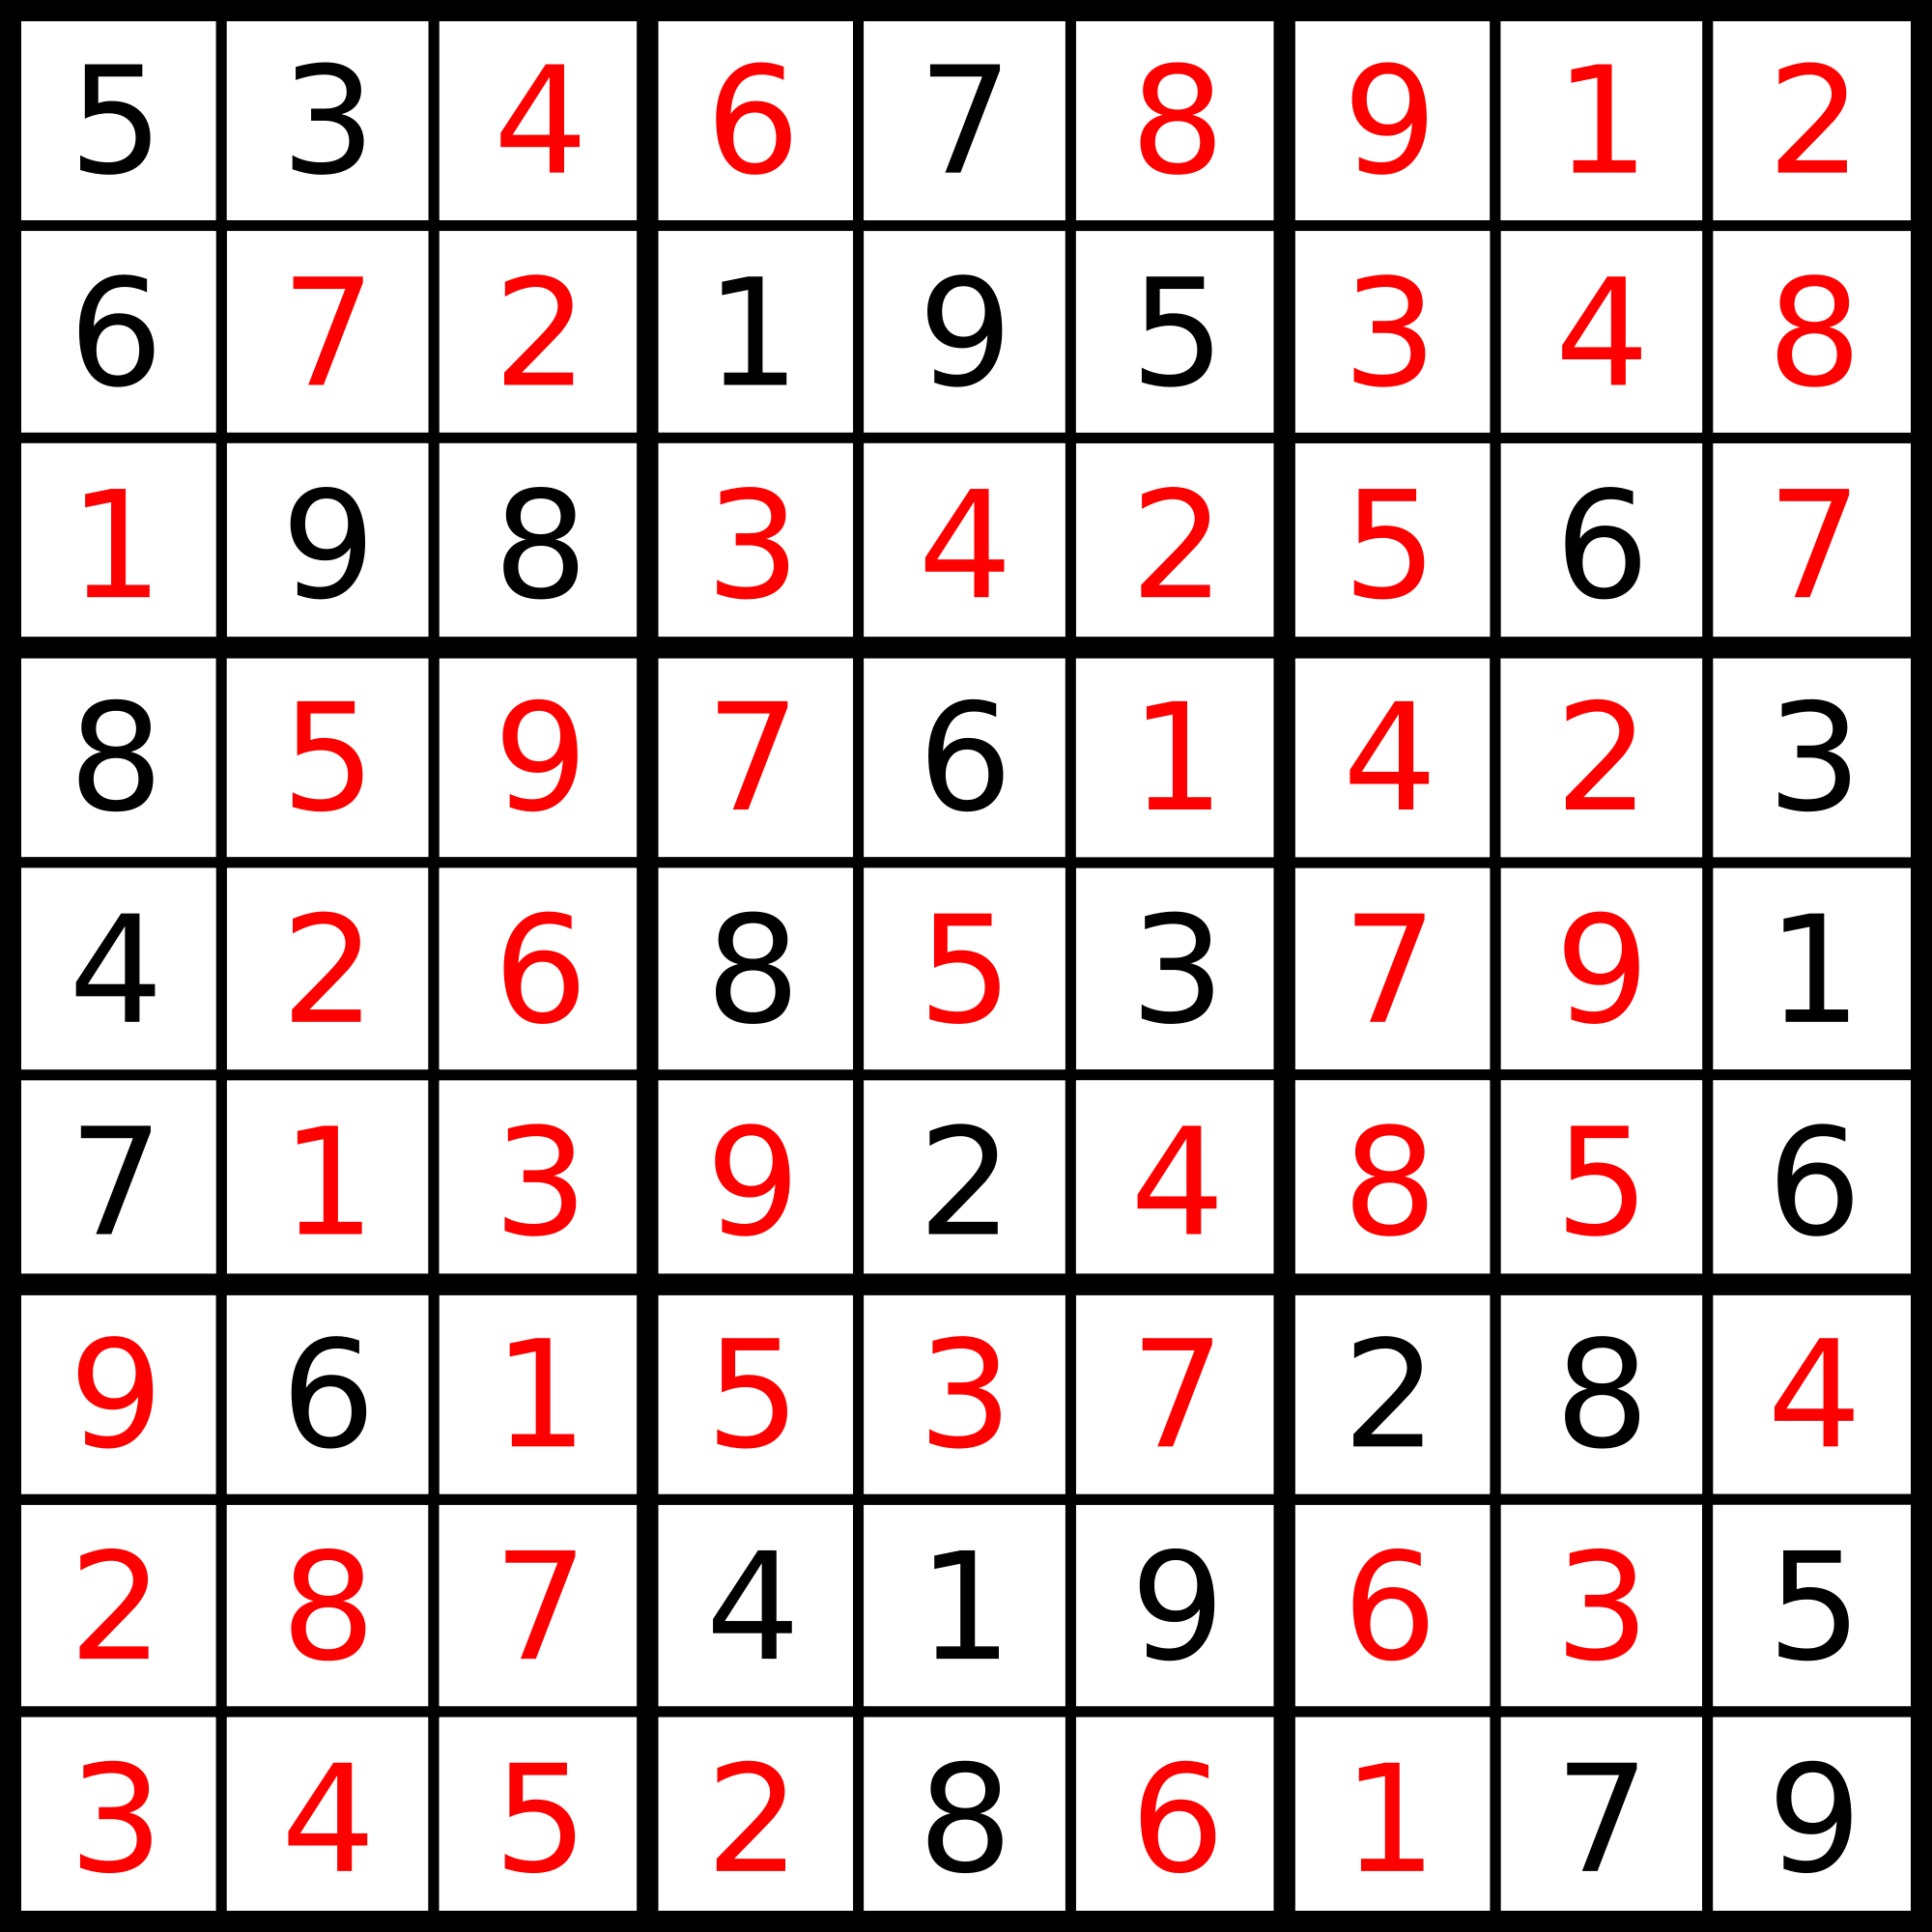
\includegraphics[width=8cm,height=8cm]{sudoku.png}
  \end{center}

}
\note[itemize]{
\item Let's say you're given a business task - how to solve Sudoku.
\item How would you do it? (suggestions hopefully not too good - $81^9$ possibilities with brute force)
\item Well, I've got a better way - use propositional logic
}

\frame{
  \parbox{\linewidth}{
    ``The term \emph{proposition} has a broad use in contemporary
    philosophy. It is used to refer to some or all of the following:
    the primary bearers of truth--value, the objects of belief and
    other ``propositional attitudes'', the referents of that--clauses
    and the meanings of declarative sentences.''
  }
}
\note[itemize]{
\item What's that? I looked on Wikipedia what a proposition is - and this is what it had to say.
\item Not very helpful!
}

\frame{
    Propositional logic is a formal way of talking about things that can be
    true or false.
}
\note[itemize]{
\item Let's think for a moment about what that means. We can start with
  things that can be true or false. Maybe when we were programming,
  we might say they had type Boolean?
}


\frame{
  \begin{center}
    $(\text{Neil went to the shops today})$\\
    $(\text{Nick started working at Football Radar in 2015})$\\
    $(\text{It's more than 30 degrees outside})$\\
    $\textbf{true}$\\
    $\textbf{false}$\\
    $a$
  \end{center}
}
\note[itemize]{
\item These are 'atomic propositions' - the smallest possible unit of propositional logic.
\item First three are simple facts - true or false.
\item We also have two constants - true or false.
\item Finally 'propositional variables' --- these are what we'll use to encode our Sudoku solution
}


\frame{
  \begin{align*}
    & \neg A  \tag{not \emph{A}}\\
    &A \wedge B \tag{\emph{A} and \emph{B}} \\
    &A \vee B \tag{\emph{A} or \emph{B}}\\
    &A \Rightarrow B \tag{if \emph{A} then \emph{B}}\\
  \end{align*}
}
\note[itemize]{
\item not A - true when A is false and false when A is true
\item A and B - true when both A and B are true, false otherwise
\item A or B - true when one or both of A and B are true
\item A imp B - true when A is false, or B is true
}


\frame{
  \begin{center}
  $(\text{\small{It's more than 30 degrees outside}}) \Rightarrow (\text{\small{Neil
        went to the shops today}})$
  \end{center}
}
\note[itemize]{
\item Note Neil doesn't have to go to the shops for this to be true
\item It's only false if Neil didn't go to the shops, and it was more than 30 degrees outside.
\item Quick demo scala: \texttt{sbt console}
\item Note that all we're doing here is building a tree
}


\frame{
  \begin{center}
    
\includegraphics[width=8cm,height=8cm]{sudoku_empty.png}
  \end{center}
}
\note[itemize]{
\item Now we can think about how we might model Sudoku with propositional logic.
\item First we need to think about which atomic propositions we might need.
\item What facts are true or false in a Sudoku solution and describe the solution perfectly?
}

\frame{
  \begin{center}
    \emph{The cell in row $i$ and column $j$ holds the number
      $k$}\\[.5cm]
    $x_{ijk}$
  \end{center}
}
\note[itemize]{
\item These seem to fit the bill quite nicely.
}

\begin{frame}[fragile]
  \begin{Verbatim}[commandchars=\\\{\}]
\PY{k}{val} \PY{n}{props}: Seq[(Row, Col, Val, Formula)] \PY{k}{=}
  \PY{k}{for} \PY{o}{\PYZob{}}
    \PY{n}{row} \PY{k}{\PYZlt{}\PYZhy{}} \PY{l+m+mf}{1.}\PY{n}{to}\PY{o}{(}\PY{l+m+mi}{9}\PY{o}{)}
    \PY{n}{col} \PY{k}{\PYZlt{}\PYZhy{}} \PY{l+m+mf}{1.}\PY{n}{to}\PY{o}{(}\PY{l+m+mi}{9}\PY{o}{)}
    \PY{n}{value} \PY{k}{\PYZlt{}\PYZhy{}} \PY{l+m+mf}{1.}\PY{n}{to}\PY{o}{(}\PY{l+m+mi}{9}\PY{o}{)}
  \PY{o}{\PYZcb{}} \PY{k}{yield} \PY{o}{(}
    \PY{n}{row}\PY{o}{,}
    \PY{n}{col}\PY{o}{,}
    \PY{n}{value}\PY{o}{,}
    \PY{n}{propVar}\PY{o}{(}\PY{l+s}{s\PYZdq{}}\PY{l+s+si}{\PYZdl{}\PYZob{}}\PY{n}{row}\PY{l+s+si}{\PYZcb{}}\PY{l+s}{\PYZus{}}\PY{l+s+si}{\PYZdl{}\PYZob{}}\PY{n}{col}\PY{l+s+si}{\PYZcb{}}\PY{l+s}{\PYZus{}}\PY{l+s+si}{\PYZdl{}\PYZob{}}\PY{n}{value}\PY{l+s+si}{\PYZcb{}}\PY{l+s}{\PYZdq{}}\PY{o}{)}
  \PY{o}{)}
\end{Verbatim}
\end{frame}
\note[itemize]{
\item This is how we might do it in Scala.
\item We store the row, col and value to let us select matching propositions later.
}

\frame{
  \begin{center}
    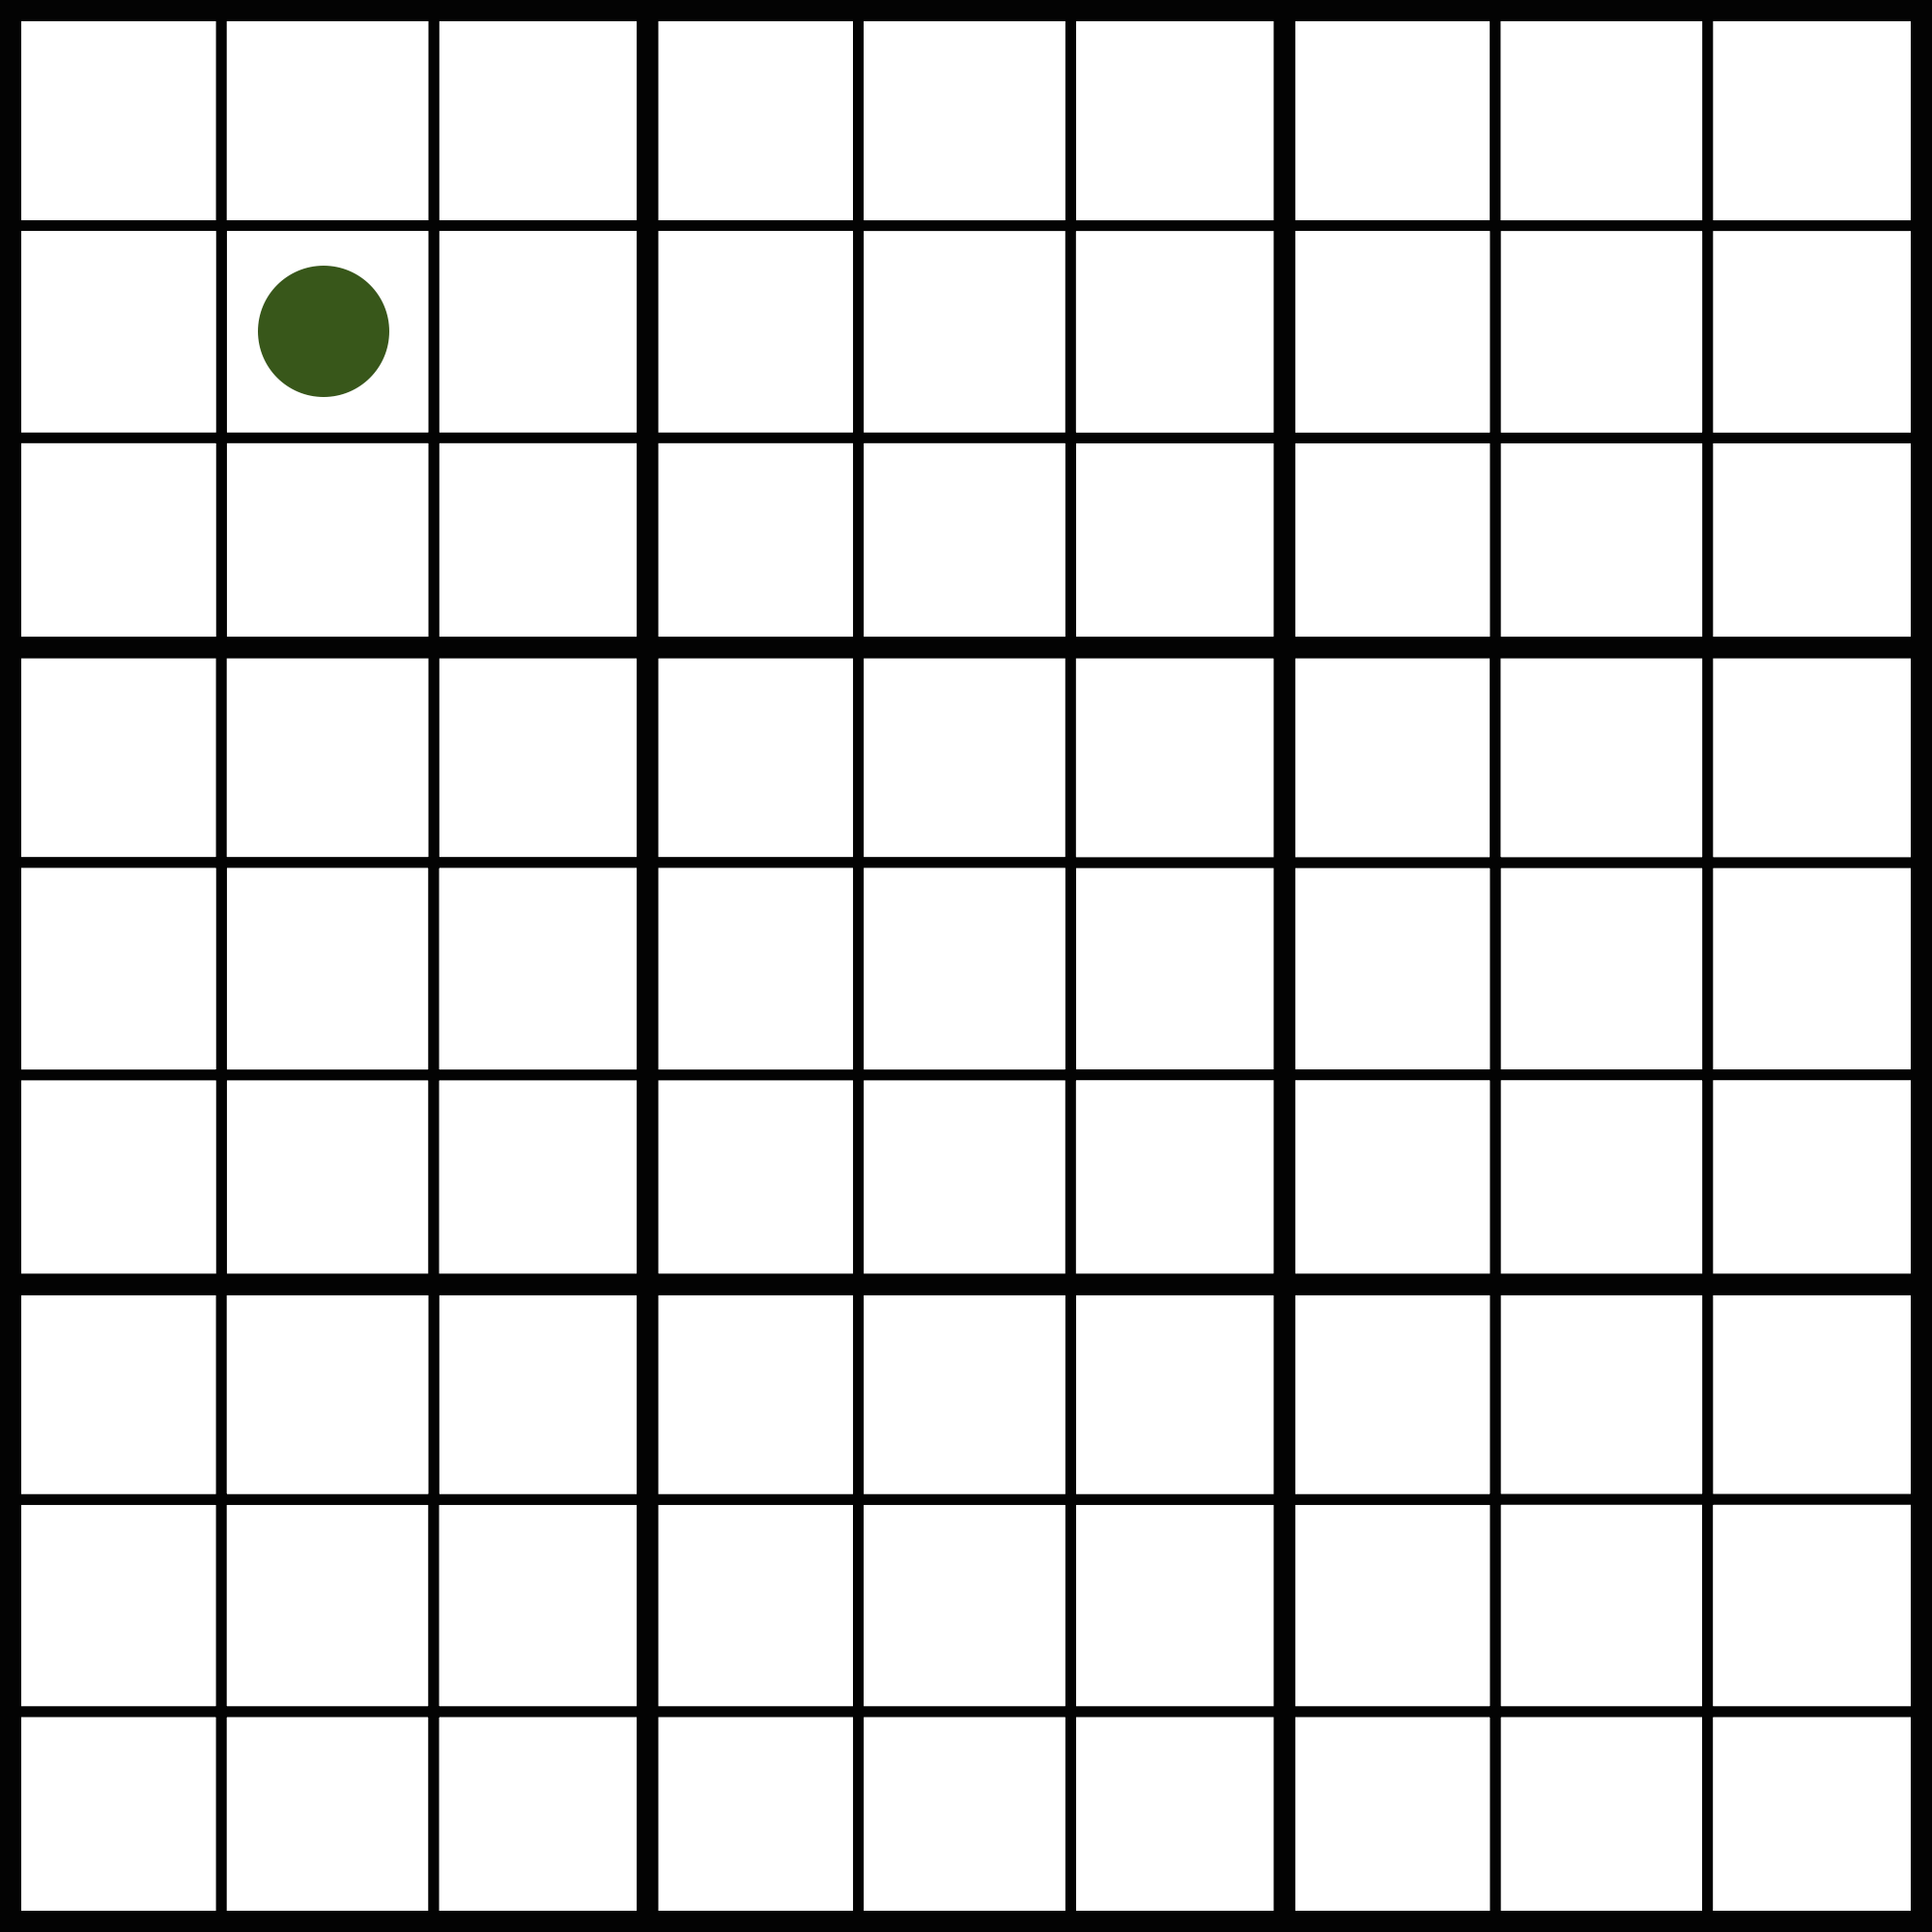
\includegraphics[width=8cm,height=8cm]{sudoku_single_cell.png}
  \end{center}
}
\note[itemize]{
\item Now we're going to try and build up a formula is true only if a Sudoku has a solution.
\item So we need to think about things that constrain what could possibly be in each cell.
}

\begin{frame}[fragile]
\begin{Verbatim}[commandchars=\\\{\}]
\PY{k}{def} \PY{n}{all}\PY{o}{(}\PY{n}{fs}\PY{k}{:} \PY{k+kt}{Iterable}\PY{o}{[}\PY{k+kt}{Formula}\PY{o}{]}\PY{o}{)}\PY{k}{:} \PY{k+kt}{Formula} \PY{o}{=}
  \PY{n}{fs}\PY{o}{.}\PY{n}{reduce}\PY{o}{(}\PY{k}{\PYZus{}} \PY{o}{\PYZam{}\PYZam{}} \PY{k}{\PYZus{}}\PY{o}{)}

\PY{k}{def} \PY{n}{any}\PY{o}{(}\PY{n}{fs}\PY{k}{:} \PY{k+kt}{Iterable}\PY{o}{[}\PY{k+kt}{Formula}\PY{o}{]}\PY{o}{)}\PY{k}{:} \PY{k+kt}{Formula} \PY{o}{=}
  \PY{n}{fs}\PY{o}{.}\PY{n}{reduce}\PY{o}{(}\PY{k}{\PYZus{}} \PY{o}{||} \PY{k}{\PYZus{}}\PY{o}{)}

\PY{k}{def} \PY{n}{eachProp}\PY{o}{(}
  \PY{n}{f}\PY{k}{:} \PY{o}{(}\PY{o}{(}\PY{k+kt}{Row}\PY{o}{,} \PY{k+kt}{Col}\PY{o}{,} \PY{k+kt}{Value}\PY{o}{,} \PY{k+kt}{Formula}\PY{o}{)}\PY{o}{)} \PY{k}{=\PYZgt{}} \PY{k+kt}{Formula}
\PY{o}{)}\PY{k}{:} \PY{k+kt}{Formula} \PY{o}{=} \PY{n}{all}\PY{o}{(}\PY{n}{props}\PY{o}{.}\PY{n}{map}\PY{o}{(}\PY{n}{f}\PY{o}{)}\PY{o}{)}
\end{Verbatim}
\end{frame}
\note[itemize]{
\item These three little helpers will help us:
\item The first just puts $\wedge$ between every formula in a list of formulae
\item The second just puts $\vee$ between every formula in a list of formulae
\item The third lets us say something must be true for every combination of (row, col, value).
}

\frame{
  \begin{center}
    \emph{If the value of row $i$ and column $j$ is $k$, then $k$ must not appear in the same row}\\[.1cm]
    \begin{gather*}
      (x_{i11} \Rightarrow \neg(x_{i21} \vee x_{i31} \vee \ldots))\\
      \wedge\\
      (x_{i12} \Rightarrow \neg(x_{i22} \vee x_{i32} \vee \ldots))\\
      \wedge\\
      \ldots\\
      \wedge\\
      (x_{i21} \Rightarrow \neg(x_{i11} \vee x_{i31} \vee \ldots))\\
      \wedge\\
      \ldots
    \end{gather*}
  \end{center}
}
\note[itemize]{
\item This isn't so bad - it's pretty much just the rule that we talked about earlier with rows, but in a more formal form.
}

\begin{frame}[fragile]
\begin{Verbatim}[commandchars=\\\{\}]
\PY{k}{val} \PY{n}{rowValueOnlyOccursOnce}: Formula \PY{k}{=}
  \PY{n}{eachProp} \PY{o}{\PYZob{}} \PY{k}{case} \PY{o}{(}\PY{n}{row}\PY{o}{,} \PY{n}{col}\PY{o}{,} \PY{n}{value}\PY{o}{,} \PY{n}{prop}\PY{o}{)} \PY{k}{=\PYZgt{}}
    \PY{n}{prop} \PY{o}{===\PYZgt{}} \PY{o}{!}\PY{n}{any}\PY{o}{(}
      \PY{k}{for} \PY{o}{\PYZob{}}
        \PY{o}{(}\PY{n}{row\PYZus{}}\PY{o}{,} \PY{n}{col\PYZus{}}\PY{o}{,} \PY{n}{value\PYZus{}}\PY{o}{,} \PY{n}{prop\PYZus{}}\PY{o}{)} \PY{k}{\PYZlt{}\PYZhy{}} \PY{n}{props}
        \PY{k}{if} \PY{n}{row\PYZus{}} \PY{o}{==} \PY{n}{row}
        \PY{k}{if} \PY{n}{col\PYZus{}} \PY{o}{!=} \PY{n}{col}
        \PY{k}{if} \PY{n}{value\PYZus{}} \PY{o}{==} \PY{n}{value}
      \PY{o}{\PYZcb{}} \PY{k}{yield} \PY{n}{prop\PYZus{}}
    \PY{o}{)}
  \PY{o}{\PYZcb{}}
\end{Verbatim}
\end{frame}
\note[itemize]{
\item This is how we might express it in Scala.
}

\frame{
  \begin{center}
    \emph{... and the same for columns...}
  \end{center}
}

\frame{
  \begin{center}
    \emph{If the value of row $i$ and column $j$ is $k$, then $k$ must not appear in the same square}
  \end{center}
}

\begin{frame}[fragile]
\begin{Verbatim}[commandchars=\\\{\}]
\PY{k}{def} \PY{n}{inSameSquare}\PY{o}{(}\PY{n}{a}\PY{k}{:} \PY{k+kt}{Int}\PY{o}{,} \PY{n}{b}\PY{k}{:} \PY{k+kt}{Int}\PY{o}{)}\PY{k}{:} \PY{k+kt}{Boolean} \PY{o}{=}
  \PY{o}{(}\PY{o}{(}\PY{n}{a} \PY{o}{\PYZhy{}} \PY{l+m+mi}{1}\PY{o}{)} \PY{o}{/} \PY{l+m+mi}{3}\PY{o}{)} \PY{o}{==} \PY{o}{(}\PY{o}{(}\PY{n}{b} \PY{o}{\PYZhy{}} \PY{l+m+mi}{1}\PY{o}{)} \PY{o}{/} \PY{l+m+mi}{3}\PY{o}{)}

\PY{k}{val} \PY{n}{squareValueOnlyOccursOnce}: Formula \PY{k}{=}
  \PY{n}{eachProp} \PY{o}{\PYZob{}} \PY{k}{case} \PY{o}{(}\PY{n}{row}\PY{o}{,} \PY{n}{col}\PY{o}{,} \PY{n}{value}\PY{o}{,} \PY{n}{prop}\PY{o}{)} \PY{k}{=\PYZgt{}}
    \PY{n}{prop} \PY{o}{===\PYZgt{}} \PY{o}{!}\PY{n}{any}\PY{o}{(}
      \PY{k}{for} \PY{o}{\PYZob{}}
        \PY{o}{(}\PY{n}{row\PYZus{}}\PY{o}{,} \PY{n}{col\PYZus{}}\PY{o}{,} \PY{n}{value\PYZus{}}\PY{o}{,} \PY{n}{prop\PYZus{}}\PY{o}{)} \PY{k}{\PYZlt{}\PYZhy{}} \PY{n}{props}
        \PY{k}{if} \PY{n}{inSameSquare}\PY{o}{(}\PY{n}{row\PYZus{}}\PY{o}{,} \PY{n}{row}\PY{o}{)}
        \PY{k}{if} \PY{n}{inSameSquare}\PY{o}{(}\PY{n}{col\PYZus{}}\PY{o}{,} \PY{n}{col}\PY{o}{)}
        \PY{k}{if} \PY{n}{row\PYZus{}} \PY{o}{!=} \PY{n}{row} \PY{o}{||} \PY{n}{col\PYZus{}} \PY{o}{!=} \PY{n}{col}
        \PY{k}{if} \PY{n}{value\PYZus{}} \PY{o}{==} \PY{n}{value}
      \PY{o}{\PYZcb{}} \PY{k}{yield} \PY{n}{prop\PYZus{}}
    \PY{o}{)}
  \PY{o}{\PYZcb{}}
\end{Verbatim}
\end{frame}
\note[itemize]{
\item We can adapt the row and column ones for this square one.
\item Here we're just using \texttt{inSameSquare} which tells us given two x or y coordinates if they are in the same square.
\item Other than that it looks pretty much the same.
}


\frame{
  \begin{center}
    \emph{The cell in row $i$ and column $j$ must hold some number}\\[.2cm]
    \begin{gather*}
      (x_{111} \vee x_{112} \vee x_{113} \vee \ldots \vee x_{119})\\
      \wedge\\
      (x_{121} \vee x_{122} \vee x_{123} \vee \ldots \vee x_{129})\\
      \wedge\\
      \ldots\\
      \wedge\\
      (x_{991} \vee x_{992} \vee x_{993} \vee \ldots \vee x_{999})
    \end{gather*}
  \end{center}
}
\note[itemize]{
\item If we try and find a solution to the formula we've built so far, we might not get what we want!
\item All $x_{ijk}$ false is a solution but not a very interesting one.
}


\begin{frame}[fragile]
\begin{Verbatim}[commandchars=\\\{\}]
\PY{k}{val} \PY{n}{eachCellHoldsValue}: Formula \PY{k}{=} \PY{n}{all} \PY{o}{\PYZob{}}
  \PY{k}{val} \PY{n}{cellProps} \PY{k}{=}
    \PY{n}{props}\PY{o}{.}\PY{n}{groupBy} \PY{o}{\PYZob{}} \PY{k}{case} \PY{o}{(}\PY{n}{row}\PY{o}{,} \PY{n}{col}\PY{o}{,} \PY{k}{\PYZus{}}\PY{o}{,} \PY{k}{\PYZus{}}\PY{o}{)} \PY{k}{=\PYZgt{}}
      \PY{o}{(}\PY{n}{row}\PY{o}{,} \PY{n}{col}\PY{o}{)}
    \PY{o}{\PYZcb{}}\PY{o}{.}\PY{n}{values}
      \PY{o}{.}\PY{n}{map} \PY{o}{\PYZob{}} \PY{n}{propsWithMetadata} \PY{k}{=\PYZgt{}}
        \PY{n}{propsWithMetadata}\PY{o}{.}\PY{n}{map} \PY{o}{\PYZob{}} \PY{k}{case} \PY{o}{(}\PY{k}{\PYZus{}}\PY{o}{,} \PY{k}{\PYZus{}}\PY{o}{,} \PY{k}{\PYZus{}}\PY{o}{,} \PY{n}{prop}\PY{o}{)} \PY{k}{=\PYZgt{}}
          \PY{n}{prop}
        \PY{o}{\PYZcb{}}
      \PY{o}{\PYZcb{}}
  \PY{n}{cellProps}\PY{o}{.}\PY{n}{map}\PY{o}{(}\PY{n}{any}\PY{o}{)}
\PY{o}{\PYZcb{}}
\end{Verbatim}
\end{frame}
\note[itemize]{
\item This one's a bit different - we just pick all the value propositions for a given row and col and $\vee$ them together.
}


\begin{frame}[fragile]
\begin{Verbatim}[commandchars=\\\{\}]
\PY{k}{val} \PY{n}{model}: Formula \PY{k}{=} \PY{n}{rowValueOnlyOccursOnce} \PY{o}{\PYZam{}\PYZam{}}
  \PY{n}{colValueOnlyOccursOnce} \PY{o}{\PYZam{}\PYZam{}}
  \PY{n}{squareValueOnlyOccursOnce} \PY{o}{\PYZam{}\PYZam{}}
  \PY{n}{eachCellHoldsValue}
\end{Verbatim}
\end{frame}
\note[itemize]{
\item Now we can build our model by $\wedge$ing all of our 'rule formulae' together.
}


\frame{
  \begin{center}
    $x_{118} \wedge x_{323} \wedge x_{237} \wedge \ldots \wedge x_{794}$
  \end{center}
}
\note[itemize]{
\item \url{http://www.telegraph.co.uk/news/science/science-news/9359579/Worlds-hardest-sudoku-can-you-crack-it.html}
\item To solve a given instance of the puzzle, we also need to say that the propositions corresponding to some partial solution are true.
\item That one's not so interesting so I've omitted it.
}


\begin{frame}[fragile]
\begin{Verbatim}[commandchars=\\\{\}]
\PY{k}{val} \PY{n}{model}: Formula \PY{k}{=} \PY{n}{rowValueOnlyOccursOnce} \PY{o}{\PYZam{}\PYZam{}}
  \PY{n}{colValueOnlyOccursOnce} \PY{o}{\PYZam{}\PYZam{}}
  \PY{n}{squareValueOnlyOccursOnce} \PY{o}{\PYZam{}\PYZam{}}
  \PY{n}{eachCellHoldsValue} \PY{o}{\PYZam{}\PYZam{}}
  \PY{n}{partialSolutionMustBeFilledIn}
\end{Verbatim}
\end{frame}
\note[itemize]{
\item This is the final overall formula we've constructed.
\item Remember, this is just a big tree of things $\neg$ed, $\wedge$ed and $\vee$ed together.
}


\begin{frame}
  \begin{center}
  A \emph{satisfying assignment} of \texttt{model} is a set of
  $x_{ijk}$ such that the overall proposition \texttt{model} is
  true.
  \end{center}
\end{frame}
\note[itemize]{
\item If we can find this satisfying assignment it will tell us the solution to the puzzle!
\item We just look for the $x_{ijk}$ that are true - there should be one for every cell and
  $k$ is the value for that cell.
}


\begin{frame}
  \begin{center}
    We can use a piece of software (a \emph{\textsc{sat} solver}) to find such an assignment
  \end{center}
\end{frame}
\note[itemize]{
\item This is a very tricky piece of software to write. Perhaps even harder than writing a sudoku solver!
\item But luckily someone else has written one for you.
}

\begin{frame}
  \begin{center}
    \vspace{0.3in}
    
\includegraphics[width=8cm]{logo-white.png}\\
    \url{https://engineering.footballradar.com}\\
    \url{@fr_devs}
  \end{center}
\end{frame}

\end{document}
